\documentclass[12pt]{article}
\usepackage{geometry}
\usepackage{amsmath}
\usepackage{amsthm}
\usepackage{amssymb}
\usepackage{mathrsfs}
\usepackage{parskip}
\usepackage{enumerate}
\usepackage{stmaryrd}
\usepackage{listings}
\usepackage{fullpage}
\usepackage[x11names, rgb]{xcolor}
\usepackage[utf8]{inputenc}
\usepackage{tikz}
\usetikzlibrary{snakes,arrows,shapes}

\begin{document}

\title{CS 360 Notes}
\author{Matthew Visser}
\date{Oct 27, 2011}
\maketitle

\section{PDA}

\subsection{Instantaneous Description}

Recall from before.
\[
(q,z,\gamma) \vdash_p (p,w,\alpha)
\]
\[
(q,x,\beta) \vdash_p^* (p,w,\alpha)
\]
We can go from $(q,x,\beta)$ to $(q',x',\alpha)$ in a finite number of steps.

One thing to know about PDAs is that they can run for ever.

\[
I \vdash_p^* J
\]

\textbf{Base case}:  $I \vdash_p^* I$
\textbf{Inductive case}:  If $I \vdash_p^* K$ and $K \vdash_p^* J$ Then $I
\vdash_p^* I$.

A \emph{valid computation} in a PDA $P$ is a sequence of instantaneous
descriptions $K_1, K_2,\dots,K_n$ where $K_1\vdash_p
K_2\vdash_p\dots\vdash_pK_n$.

If a computation is valid for $P$; then it remains valid if we add the string
$\gamma \in \Gamma^*$ to the end of the stack for all instantaneous descriptions
in the computation.

If a computation is valid for a PDA $P$ then it remains valid if we add the
string $u \in \Sigma^*$ to the end of the input for all instantaneous
descriptions in the computation.

\subsection{How does a PDA Accept?}

Two ways:
\begin{enumerate}
	\item \textbf{Like a DFA: at end of input, the machine is in an accepting
		state.}

		$P$ \emph{accepts} a word $x$ if $(q_0,x,Z_0) \vdash_P^*
		(q_i,\varepsilon,\alpha)$ where $q_i \in F$ for any $\alpha \in
		\Gamma^*$.
	\item \textbf{Accepting by empty stack.}

		$(q_0,x,Z_0) \vdash_{P}^{*}(q_i,\varepsilon,\varepsilon),\quad q_i \in
		Q$
\end{enumerate}

\subsection{Example}

We have the language
\[
L = \{0^i1^i\ |\ i \ge 0\}
\]



%%% Begin pda1.dot %%%
\begin{center}
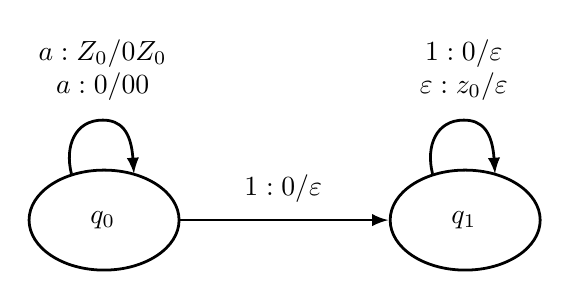
\begin{tikzpicture}[>=latex,line join=bevel,]
  \pgfsetlinewidth{1bp}
%%
% Node: q_1
\begin{scope}
  \definecolor{strokecol}{rgb}{0.0,0.0,0.0};
  \pgfsetstrokecolor{strokecol}
  \draw (160bp,18bp) ellipse (27bp and 18bp);
  \draw (159.5bp,18bp) node {$q_1$};
\end{scope}
  % Node: q_0
\begin{scope}
  \definecolor{strokecol}{rgb}{0.0,0.0,0.0};
  \pgfsetstrokecolor{strokecol}
  \draw (30bp,18bp) ellipse (27bp and 18bp);
  \draw (29.5bp,18bp) node {$q_0$};
\end{scope}
  \pgfsetcolor{black}
  % Edge: q_0 -> q_1
  \draw [->] (56.712bp,18bp) .. controls (75.608bp,18bp) and (101.35bp,18bp)  .. (132.32bp,18bp);
  \definecolor{strokecol}{rgb}{0.0,0.0,0.0};
  \pgfsetstrokecolor{strokecol}
  \draw (94.5bp,29.5bp) node {$1:0/\varepsilon$};
  % Edge: q_0 -> q_0
  \draw [->] (18.25bp,34.664bp) .. controls (15.75bp,44.625bp) and (19.5bp,54bp)  .. (29.5bp,54bp) .. controls (35.906bp,54bp) and (39.747bp,50.152bp)  .. (40.75bp,34.664bp);
  \draw (29.5bp,72bp) node {$\begin{matrix}a:Z_0/0Z_0\\a:0/00\end{matrix}$};
  % Edge: q_1 -> q_1
  \draw [->] (148.25bp,34.664bp) .. controls (145.75bp,44.625bp) and (149.5bp,54bp)  .. (159.5bp,54bp) .. controls (165.91bp,54bp) and (169.75bp,50.152bp)  .. (170.75bp,34.664bp);
  \draw (159.5bp,72bp) node {$\begin{matrix}1:0/\varepsilon \\ \varepsilon:z_0/\varepsilon\end{matrix}$};
%
\end{tikzpicture}
\end{center}
%%% end pda1.dot %%%

Justification, \dots fairly obvious (need to describe more in assignments).


\subsection{Example: Palindrome Without a Center Marker}

Last example like this we had $L = \{ w!w^R\ |\ w \in \{a,b\}^*\}$. Now we want
to have a language without the ``!''.

We have the language \[L = \{ ww^R\ |\ w \in \{a,b\}^*\}\]

We can use the nondeterministic property to ``guess'' that we are at the
midpoint each time.
%%% Begin pda2.dot %%%
\begin{center}
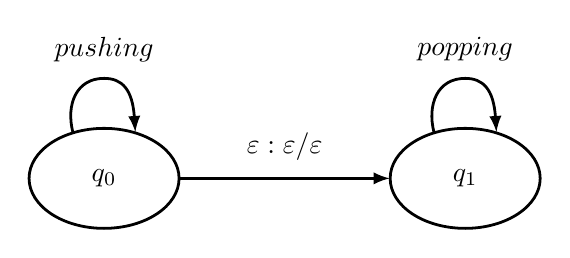
\begin{tikzpicture}[>=latex,line join=bevel,]
  \pgfsetlinewidth{1bp}
%%
\pgfsetcolor{black}
  % Edge: q_0 -> q_1
  \draw [->] (54.212bp,18bp) .. controls (73.108bp,18bp) and (98.851bp,18bp)  .. (129.82bp,18bp);
  \definecolor{strokecol}{rgb}{0.0,0.0,0.0};
  \pgfsetstrokecolor{strokecol}
  \draw (92bp,29.5bp) node {$\varepsilon:\varepsilon/\varepsilon$};
  % Edge: q_0 -> q_0
  \draw [->] (15.75bp,34.664bp) .. controls (13.25bp,44.625bp) and (17bp,54bp)  .. (27bp,54bp) .. controls (33.406bp,54bp) and (37.247bp,50.152bp)  .. (38.25bp,34.664bp);
  \draw (27bp,64.5bp) node {$pushing$};
  % Edge: q_1 -> q_1
  \draw [->] (145.75bp,34.664bp) .. controls (143.25bp,44.625bp) and (147bp,54bp)  .. (157bp,54bp) .. controls (163.41bp,54bp) and (167.25bp,50.152bp)  .. (168.25bp,34.664bp);
  \draw (157bp,64.5bp) node {$popping$};
  % Node: q_1
\begin{scope}
  \definecolor{strokecol}{rgb}{0.0,0.0,0.0};
  \pgfsetstrokecolor{strokecol}
  \draw (157bp,18bp) ellipse (27bp and 18bp);
  \draw (157bp,18bp) node {$q_1$};
\end{scope}
  % Node: q_0
\begin{scope}
  \definecolor{strokecol}{rgb}{0.0,0.0,0.0};
  \pgfsetstrokecolor{strokecol}
  \draw (27bp,18bp) ellipse (27bp and 18bp);
  \draw (27bp,18bp) node {$q_0$};
\end{scope}
%
\end{tikzpicture}
\end{center}
%%% end pda2.dot %%%

\end{document}
% vim: tw=80
